%++++++++++++++++++++++++++++++++++++++++
% Don't modify this section unless you know what you're doing!
\documentclass[letterpaper,12pt]{article}
\usepackage{float}
\usepackage[spanish]{babel}
\selectlanguage{spanish}
\usepackage[utf8]{inputenc}
\usepackage{tabularx} % extra features for tabular environment
\usepackage{amsmath}  % improve math presentation
\usepackage{graphicx, wrapfig, subcaption, setspace, booktabs}
\usepackage{graphicx} % takes care of graphic including machinery

\usepackage[margin=1in,letterpaper]{geometry} % decreases margins
\usepackage{cite} % takes care of citations
\usepackage[final]{hyperref} % adds hyper links inside the generated pdf file
\usepackage{amsmath}
\usepackage{amssymb}
\usepackage{enumerate}
\usepackage{url}
\hypersetup{
	colorlinks=true,       % false: boxed links; true: colored links
	linkcolor=blue,        % color of internal links
	citecolor=blue,        % color of links to bibliography
	filecolor=magenta,     % color of file links
	urlcolor=blue         
}
%++++++++++++++++++++++++++++++++++++++++


\begin{document}

\title{Reporte de la actividad 5}
\author{Daniela Olmos Velderrain\\Grupo 3}
\date{28 de febrero de 2019}

\maketitle

\section{Introducción}
En esta actividad utilizamos datos de temperatura y precipitación del municipio de Cajeme para determinar los efectos del Cambio Climático en dicha región.
\\
\\
Los datos empleados fueron adquiridos de la página del Servicio Meteorológico Nacional de la Comisión Nacional del Agua.
\\
\\
Se calcularon 16 índices que son indicadores de los efectos del Cambio Climático para la región elegida, los cuales se basan en los registros de precipitación y temperatura de la zona. 
\\
\\
\section{Desarrollo}
\subsection{Metodología} 
El manejo de los datos del archivo fue similar al de las actividades pasadas. Se descargaron las librerías necesarias para el análisisde datos y visualización:

\begin{verbatim}
import pandas as pd
import numpy as np
import matplotlib.pyplot as plt
\end{verbatim}

Ya que los índices solicitados se debían calcular por años o por meses, era necesario tener estas dos variables como parte de nuestro Data Frame. Como el archivo cuenta con una columna de fechas, a esta se le dio formato de fecha mediante:
\begin{verbatim}
    df['FECHAN'] = pd.to_datetime(df.apply(lambda x: x['FECHA'], 1), dayfirst=True)
    
    df = df.drop(['FECHA'], 1)
\end{verbatim}

Para poder definir columnas para meses y años, estos se extrajeron de la nueva variable "FECHAN".

\begin{verbatim}
df['MES'] = df['FECHAN'].dt.month
df['AÑO'] = df['FECHAN'].dt.year
\end{verbatim} 

Debido a que en ocasiones los registros de datos están incompletos, ya que pueden llegar a haber días y meses de datos faltantes, se contaron los datos del archivo por año, para determinar el porcentaje de datos de cada uno:

\begin{verbatim}
df2 = pd.DataFrame(df.groupby('AÑO').count())
df2 = df2.filter(['PRECIP'],axis=1)
df2 = df2.reset_index()

for i in range(0,len(df2)):
    NumDatos = df2["PRECIP"][i]-1
    print("Año:", df2['AÑO'][i], "Núm dat:", NumDatos, ", Porcentaje:",
    np.round((NumDatos*100)/365.0, decimals=2), "%")
\end{verbatim}

Para calcular índices como el número de días con heladas, días de verano, entre otros, fue importante el empleo de las funciónes $count$ y  $groupby$, ya que una vez restringido el Data Frame a los valores que cumplían con la condición indicada, estas funciones nos permitieron agrupar los datos por año y contarlos. Esto se puede apreciar en el cálculo del número de días con heladas por año:

\begin{verbatim}
#Tomar temperaturas TMIN menores a 0
nHel = pd.DataFrame(df.loc[df['TMIN']<0])

#Agrupar por año y contar datos 
nHel = pd.DataFrame(nHel.groupby('AÑO').count())
\end{verbatim}

El uso de arreglos y loops también fue vital para realizar el análisis de los datos, ya que en muchas ocasiones estos debían ser revisados cada año y cada mes, lo cual habría sido muy ineficiente de haberlo realizado a pie.

Otras funciones que conocimos en las actividades anteriores, y fueron muy útiles en este trabajo fueron $max$, $min$ y $mean$, ya que estas permitieron calcular indicadores que tuvieran que ver con máximos y mínimos mensuales de temperatura o precipitación, así como promedios de temperaturas. 

El uso de estos elementos se puede ejemplificar con el cálculo de la máxima mensual de la temperatura máxima:

 \begin{verbatim}
     TXx=[]
inicial=df['AÑO'][0]
nAños=df['AÑO'].nunique()

#El primer loop crea un DataFrame del año
for i in range(0,nAños):
        daño = df[df['AÑO']==inicial]
        #El segundo loop crea un DataFrame por mes
        for j in range (1,13):
                dmes = daño[daño['MES']==j]
                #Se busca la máxima de Tmax 
                TmaxMes = dmes.TMAX.max()
                TXx.append(TmaxMes)    
        inicial=inicial+1

 \end{verbatim}


\subsection{Resultados}
A continuación se muestra una visualización de cada uno de los índices calculados.


\begin{center}
	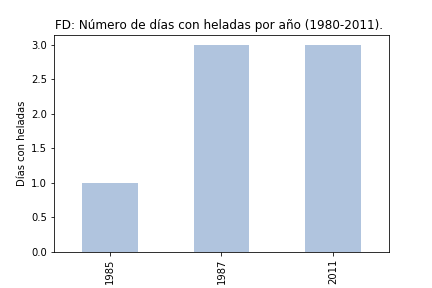
\includegraphics[height=5cm]{grafica1.png}\hspace*{\fill}
	\label{graf1}
   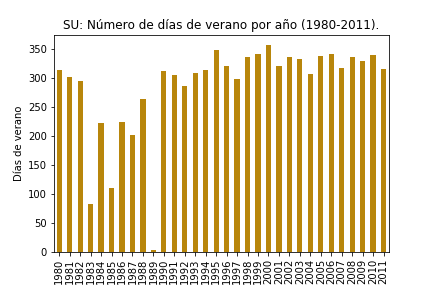
\includegraphics[height=5cm]{grafica2.png}
    \label{graf2}
\end{center}

\begin{center}
	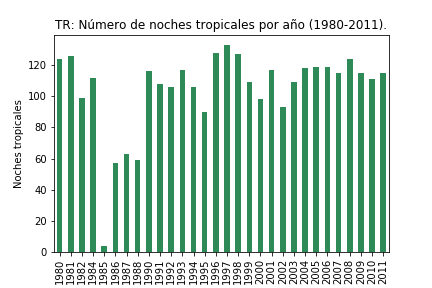
\includegraphics[height=5cm]{grafica3.png}
	\label{graf3}
\end{center}

Las grafica de FD muestra el número de días en que la temperatura mínima fue menor a $0^\circ C$, lo cual no ocurre con mucha frecuencia como se puede observar, ya que Cajeme es un municipio cálido. Por otra parte, las gráficas de SU y TR muestran el número de días de verano (cuando la temperatura máxima fue mayor de $25^\circ C$) y el número de noches tropicales (cuando la temperatura mínima fue mayor a $20^\circ C$). Estos parámetros sí se cumplen con más frecuencia en esta cálida región y parecen mantenerse altos para todos los años. En los años donde estos dos indicadores son muy bajos probablemente se deba a la falta de datos, ya que en 1989 (el año más bajo para estos índices) solo se cuenta con el 8.22\% del total de días del año.
\\
\\


\begin{figure}[H]
\centering
\fbox{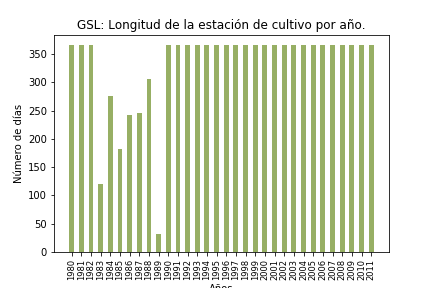
\includegraphics[width=0.5\linewidth]{grafica4.png}}
\label{graf4}
\end{figure}

En la gráfica de GSL se muestra el periodo entre los primeros 6 días seguidos del año con temperatura promedio mayor a $5^\circ C$, y los últimos 6 días seguidos del año con temperatura promedio menor a $5^\circ C$. Pareciera que la gráfica es uniforme, a excepción de temporadas de cultivo extrañamente cortas. Esto es debido a la falta de datos en el registro de dichos años (además de 1989, otros años como 1983 y 1985 cuentan solo con el 32.6\% y 49.59\% de los datos). La temporada de cultivo dura todo el año en Cajeme, ya que por ser zona tropical la temperatura promedio rara vez baja de los $0^\circ C$, haciéndolo un lugar muy propicio para la siembra.


\\
\\

\begin{center}
	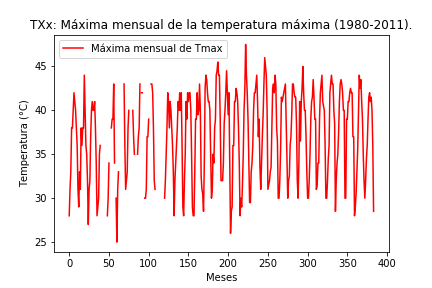
\includegraphics[height=5cm]{grafica5.png}\hspace*{\fill}
	\label{graf5}
   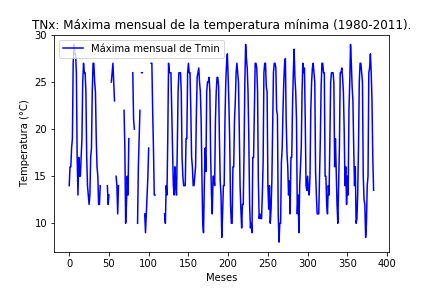
\includegraphics[height=5cm]{grafica6.png}
    \label{graf6}
\end{center}

En las gráficas de TXx y TNx observamos como varían las máximas mensuales de temperatura máxima y mínima a través de los años. Estas gráficas parecen oscilar, y podemos interpretar esta oscilación como la variación de la temperatura a través de las estaciones de un año. De la gráfica de TXx podemos decir que en Cajeme se han llegado a alcanzar temperaturas incluso mayores a $45^\circ C$ en las últimas décadas.
Por otra parte, en la gráfica de TNx,la temperatura mínima sube a valores máximos cercanos a  $30^\circ C$. 


\begin{center}
	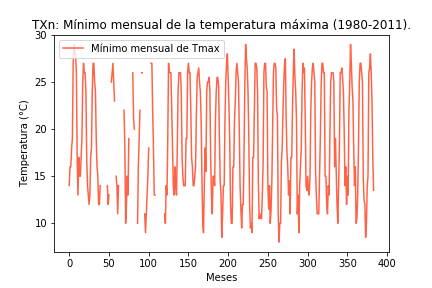
\includegraphics[height=5cm]{grafica7.png}\hspace*{\fill}
	\label{graf7}
   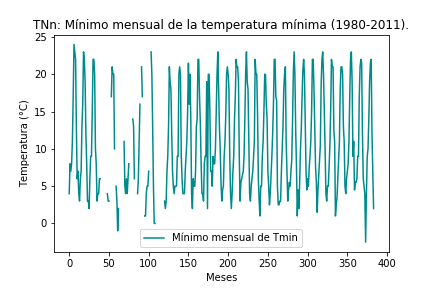
\includegraphics[height=5cm]{grafica8.png}
    \label{graf8}
\end{center}

En las gráficas de TXn y TNn se observa un comportamiento similar al de las gráficas anteriores. Se ve en TXn que el mínimo de de la temperatura máxima para los meses más calientes se acerca a los $30^\circ C$, y en los fríos puede llegar hasta los $10^\circ C$. En la gráfica de TNn el mímino de la temperatura mínima en los meses cálidos está entre $20\circ C$ y $25^\circ C$; en los meses fríos el mínimo se ubica entre $0^\circ C$ y $5^\circ C$.

\begin{center}
   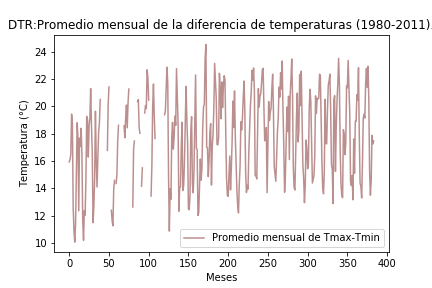
\includegraphics[height=5cm]{grafica9.png}
    \label{graf9}
\end{center}

En la gráfica de DTR se observa que la temperatura puede variar en promedio más de $20^\circ C$, y esto ha ido en aumento desde 1980. Esto quiere decir que la diferencia entre la temperatura más baja y la más cálida en un día es cada vez mayor. 

\begin{center} 
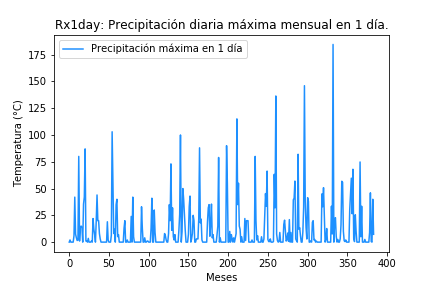
\includegraphics[height=6cm]{grafica10.png}\hspace*{\fill}
	\label{graf10}
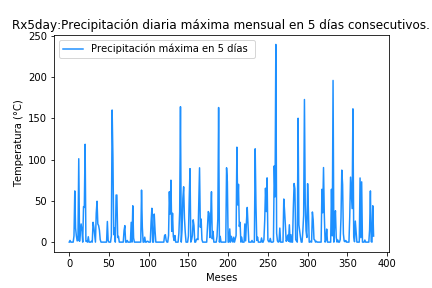
\includegraphics[height=6cm]{grafica11.png}
    \label{graf11}
\end{center}

En las gráficas de Rx1day y Rx5day podemos observar la mayor cantidad de precipitación que hubo en un día del mes o en un periodo de 5 días en un mes. En ellas podemos interpretar que los picos se encuentran en los meses lluviosos de cada año. Podemos notar, especialmente en Rx1day, que la cantidad de lluvia va en aumento para estos periodos de tiempo, lo cual puede sugerir que las lluvias son cada vez más potentes. 


\begin{center}
	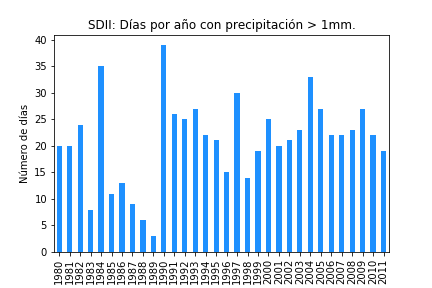
\includegraphics[height=6cm]{grafica12.png}\hspace*{\fill}
	\label{graf12}
   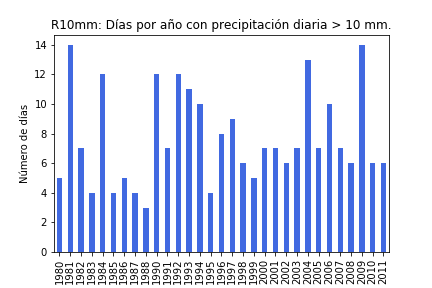
\includegraphics[height=6cm]{grafica13.png}
    \label{graf13}
\end{center}

\begin{center}
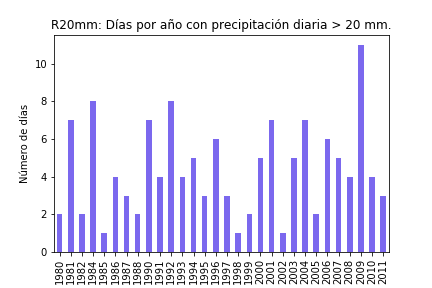
\includegraphics[height=6cm]{grafica14.png}
    \label{graf14}
\end{center}

Las gráficas de SDII, R10mm y R20mm nos indican los días por año en que la precipitación fue mayor que 1, 10 y 20 milímetros. En SDII notamos que pueden presentarse fácilmente más de 20 días en el año con lluvia, pero al subir el parámetro a 10 y 20 mm vemos que son cada vez menores los días que cumplen este requisito, y los valores aumentan con el paso del tiempo. Podemos interpretar esto como el aumento en las lluvias torrenciales, ya que es cada vez mayor la cantidad de precipitación que puede presentarse en un solo día.

\begin{center}
   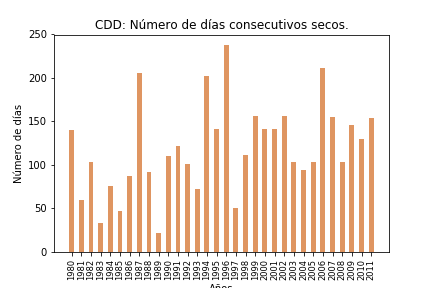
\includegraphics[height=6cm]{grafica15.png}\hspace*{\fill}
   \label{graf15}
   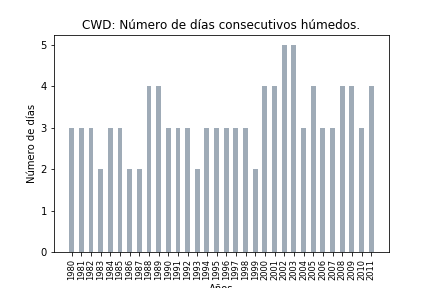
\includegraphics[height=6cm]{grafica16.png}
   \label{graf16}
\end{center}

En las gráficas de CDD y CWD se registraron el número de días consecutivos secos (de precipitación menor a 1mm) y de fías húmedos (con precipitaciones mayores a 1mm) para cada año. Por ser un lugar cálido y poco lluvioso, Cajeme presenta gran cantidad de días consecutivos secos en cada año, llegando fácilmente a más de 100 de estos en un año. En CWD notamos que el número de días consecutivos húmedos ha aumentado desde 1980, pasando de 2 hasta 5 días consecutivos en 2003, con una tendencia que parece continuar hacia números cada vez mayores.



\section{Conclusiones}
De acuerdo a los indicadores calculados, el clima de Cajeme en los últimos años sigue una tendencia que parece sugerir una mayor presencia de precipitaciones en la zona. Las lluvias abuntantes y los periodos de lluvia prolongados son cada vez más frecuentes, lo cual puede atribuirse a los efectos del cambio climático en la región. 
Sin embargo, el registro de datos no es del todo confiable, ya que hay años en los que hay muchos valores faltantes. De 1983 a 1989 no se cuenta con el $100\%$ de los datos (hay varios años que tienen incluso menos del $50\%$). Esta falta de valores refleja resultados erróneos en las gráficas, lo cual puede prestarse a que se dé una mala interpretación de los índices. 
Esta falta de datos se podría complementar con los de estaciones cercanas, comparando los registros de años iguales para tener una mejor idea de los patrones de clima que tuvieron estos.

\section*{Bibliografía}
\begin{itemize}
\item Servicio Meteorológico Nacional. Recuperado el 20 de febrero del 2019 desde \\http://smn.cna.gob.mx/es/informacion-climatologica-por-estado?estado=son
\item \\Matplotlib. Recuperado el 17 de febrero de 2019 desde \\https://matplotlib.org/
\item \\Expert Team on Climate Change Detection and Indices (ETCCDI).Recuperado el 28 de febrero de 2019 desde \\http://etccdi.pacificclimate.org/list\_27\_indices.shtml
\end{itemize}


\end{document}